\chapter{Design and Implementation}
% This chapter may be called something else\ldots but in general the
% idea is that you have one (or a few) ``meat'' chapters which describe
% the work you did in technical detail.
\begin{tcolorbox}[boxsep=0mm,left=2.5mm,right=2.5mm]
    \textbf{Design and Implementation:} {\em In this section, I will outline the
    goals of my system. I will give a brief overview of the chapture structure,
    summarising each core section and what I achieve.}
\end{tcolorbox}

\section{System Architecture}
\begin{figure}[h]
    \centering
    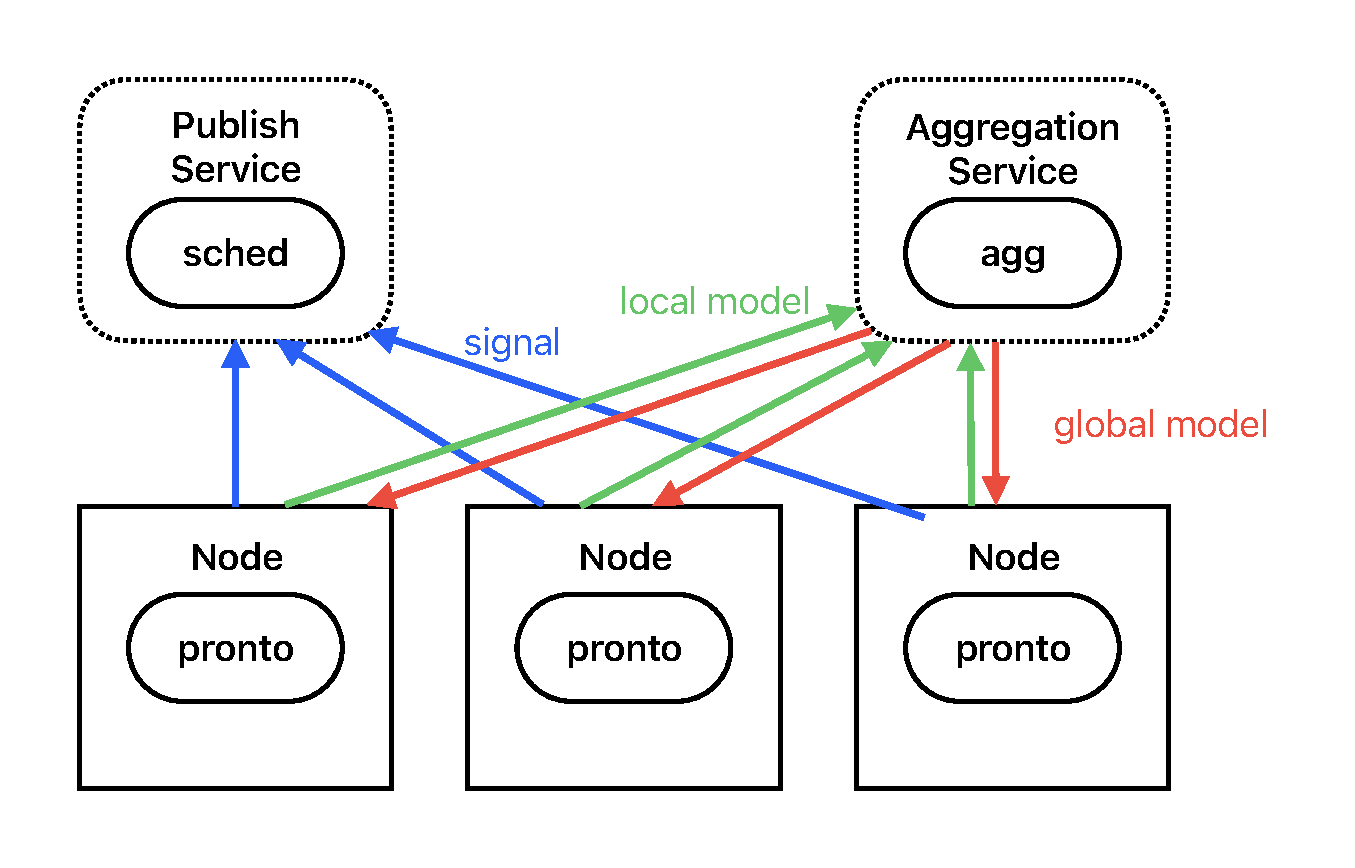
\includegraphics[width=\textwidth]{images/system.pdf}
    \caption{The components within the Pronto system}
    \label{pronto-system}
\end{figure}

The Pronto system consists of three core components (shown in figure
\ref{pronto-system}):
\begin{itemize}
    \item Pronto DaemonSet: each node in the cluster will have a pronto pod
        running on it. This pod collects telemetry of the node performance and
        generates its local model and a willigness signal. When the Pronto pod
        deems its local model outdated, it requests the latest aggregated global
        model from the Aggregation service. In addition, it periodically
        generates and publishes its willigness signal to the Publish service.
    \item Scheduler: In Pronto, the scheduler is a \textbf{Scheduler Plugin}, implementing custom
        Filter, Score and Reserve functions. It also acts as the server of the
        Publish service, collecting the latest willingness scores of each node
        which it uses in its scheduling decisions.
    \item Aggregator: This deployment provides the Aggregation service. The
        underlying \verb|pronto-agg| pod recieves local models from nodes and
        returns the latest aggregated global model.
\end{itemize}

\section{Applying Pronto For Kubernetes}

\subsection{Metric Selection}
In the paper, Pronto uses \verb|CPU-Reeady| which is generated by the VMware
vSphere virtualisation platform. This metric can't be used within a
Kubernetes cluster as machines can be both virtual and physical. Since Linux
4.20+, the kernel can track how long tasks are stalled waiting for the CPU
at a cgroup granularity. By inspecting the the root cgroup’s CPU pressure
file using \verb|cat /proc/pressure/cpu| you can measure the total time all
processes spent waiting for the CPU to be available.

While this type of metric can be used to alert of performance degradation,
this metric has a few shortcomings. Firstly, it only reports CPU-centric
information. This is not always representative measure of resource
contention as memory-heavy workloads may starve for RAM resources while
metrics like \verb|CPU-Ready| and \verb|/proc/pressure/cpu| remain
unaffected.
\begin{figure}[h]
    \centering
    
\includegraphics[width=\textwidth]{images/blank.pdf}
    \caption{The values of \texttt{/proc/pressure/cpu} during an example Kubernetes workload.}
    \label{pressure-eval}
\end{figure}
TODO: Look into why I did not use metrics like /proc/pressure/cpu. If they
are not useful, I can use them as an argument to why I used resource
utilisation and pivot to the idea of Pronto allows federated information to
help scheduling decisions. If it works, can quickly implement Pronto and
constrast

Secondly, a significant amount of resources are used starting up or deleting
containers. This results in large spikes, as shown in figure
\ref{pressure-eval}, which are difficult to distinguish from genuine CPU-Ready
spikes. As Pronto uses spike detection to predict future resource performance
degradation, container start-ups could produce detectable spikes which would
reduce the rate at which pods are assigned to nodes and could result in lower
throughput.

I decided to adapt Pronto to use fine-grained time-series measurements such as
the CPU utilisation, memory consumption to provide real-time performance data of
individual nodes as proposed in the future works section of
\cite{grammenos_pronto_2021}.

\subsection{Metric Collection}
I decided to collect CPU and memory utilisation as my telemetry data, as these
metrics are easily accessible and are used in a variety of industry-standard
schedulers \cite{hadoop2016apache,sahasrabudhe_improved_2015}.

Metric Server is a cluster-level add-on that provides near real-time CPU and
memory usage metircs for Pods and Nodes. These metrics are easily accessed through
the \verb|metrics.k8s.io/v1| APIService and are updated by the Metric Server scraper
periodically (default every 15s). This method of metric collection is not
suitable. Certain Pods may complete in less than 15 seconds and thus may not
be detected by the signal. In addition, it would take $15 \times \text{batch size}$
seconds between model updates (required to collect a single
batch before performing subspace merging), and would result in a less
representative and out-of-date model of "current" resource usage.

Instead, I decided to have a pod running on each node, scraping
metrics from files within the Linux \verb|/proc| directory.
\verb|/proc/stat| reports the cumulative count of "jiffies" (typically
hundredths of a second) each cpu spent in a specific mode \cite{proc_stat5}.
I can then calculate cpu utilisation using:
\[ \text{CPU Usage\%} = 1 - \frac{\Delta(\text{idle} +
\text{iowait}}{\Delta{\Sigma \text{all fields}}} \]
\verb|/proc/meminfo| shows a snapshot of memory usage in kilobytes. The
percentage of memory used can then be calculated from the provided fields:
\[ \text{Memory Used\%} = 1 - \frac{\text{MemFree} +
\text{Buffers} + \text{Cached}}{\text{MemTotal}}\]
Due to the higher refresh rate, we can poll these files more frequently
($\approx$ 10Hz), and can remove the network latency that would come from
making calls to the Metric Server APIService.


\subsection{Denoising and Filtering Telemetry Data}
While the modified version of Pronto that uses utilisation metrics won't perform
peak detection, the signal will still be influenced by short-lived spikes. As
mentioned in the earlier section, pod creation and deletion incurrs a visible
spike in resource usage. To prevent a non-representative local model of pod
resource utilisation, as well as a noisy willigness signal, we needed to denoise
the original metrics.
\begin{figure}[h]
    \centering
    
\includegraphics[width=\textwidth]{images/blank.pdf}
    \caption{Resource utilisation telemetry of a node during the lifecycle of a
    pod. It will have tags for when container events occured. In addition, I
    will demonstrate the effects of different filters when applied to the
    trace}
    \label{utilisation-noise}
\end{figure}
Investigation showed that the spikes caused from container events would last
$\approx$200 milliseconds. Thus when sampling at a 10Hz frequency we can use
Dynamic EMA to suppress container-event caused spikes but allow the smoothed
metric to quickly converge on the new utilisation if the spike exceeded the 300
millisecond threshold. From figure \ref{utilisation-noise}, we can see how
Dynamic EMA outperforms other low-cost filters. While more sophisticated filters
exist, they were not considered due to their higher computational cost and thus
would rob scheduled pods of the available resources. I had considered applying
the filter directly to the signal instead of the collected telemetry, but by
only filtering the signal, it would allow the local model to be polluted by
these container-event resource spikes.

TODO: Could do a more thorough investigation with a table containing event
time distribution

\section{Federated Resource Usage Model}

\subsection{Local Model Construction}
\label{sec:local-model-construction}

To build its local model, each node periodically samples its telemetry data $y
\in [0,1]^{2}$. Once it has $b$ samples, the resulting telemetry dataset $A \in
[0,1]^{2 \times b}$ is merged into the previous subspace using iterative-SVD. We
do not mean-center the telemetry data before applying SVD becuase we are
interested in the magnitude of resources rather than their changes. If we
applied standard Pronto to utilisation metrics, the creation or deletion of a
pod would result in a spike in resource usage. Even if the resource usage peaked
at 50\% utilisation, Pronto only uses peak detection and thus would detect the
spike and create a false-positive rejection signal.

The lack of mean-centering does violate the original assumptions of PCA. As
previously mentioned in section \ref{pronto-overview}, the resulting $U$ and
$\Sigma$ from the SVD of a mean-centered matrix correspond to the prinicple
components of the original matrix and the variance within the original matrix in
those directions. When we don't mean-center the telemetric data, the resulting
matrices produced by SVD have a different meaning: the resulting $U$ and
$\Sigma$ matrices correspond to the principle components of the original matrix
assuming that the mean-center was the \textbf{0} vector. In other words, $U$'s
column vectors form a basis along which maximises the sum of square distances
from projecting the telemetry data along $u_i$. Crucially, $u_i$ can be
understood as the typical directions of resource usage of a pod running on a
node.

One caveat of not mean-centering the matrix is that adding more non-zero
vector samples to the telemetry data before running SVD will increase the
resulting $\sigma_i$ values. This also applies to running iterative-SVD to merge
new samples into the local model. As $\sigma$ is used in Pronto's signal
function, and in later sections will be used in the new proposed signal, we want
to prevent the value of $\sigma$ from arbitrarily exploding. $\sigma_i$ is equal to sum of square
distances, and so scaling the concatenated matrix by $\frac{1}{\sqrt{2}}$ before
applying SVD averages the square projected distance of both matrices in all
vector directions. This results in a new "average" $\sigma$ which merges new
telemetry into the local model with a forget factor of 0.5.

\subsection{Aggregation}

The aggregation of local models to produce a global model also uses the same
iterative-SVD as defined in section \ref{sec:local-model-construction}. In
addition, instead of using a hierarchical aggregation system, I use flat
aggregation service - all aggregation requests are handled by a single node.
In the original Pronto paper, the authors assumed that there was no
communication latency. However, in a real-world cluster this assumption does not
hold. Adding additional aggregation layers would increase the overall aggregation
latency.

Instead with a aggregation server, I can reduce the overall latency of
aggregation requests. To reduce request latency further, actual model
aggregation is not performed on the request's critical path. On receipt, the local
model is enqueued to be aggregated and the latest global model is returned. A
background thread iterative-SVD merges the queued local models into the global
model. In summary, this system trades consistency for latency and throughput,
which becomes a dominant factor when scaling to hundreds of nodes.

TODO: Investigate the latency of throughput/limit of the aggregation server.
TODO: Could have multiple aggregation server pods with a load balancer. Could
then have these servers periodically share with eachother their latest models to
converge.

\subsection{Rejection Signal}
\begin{tcolorbox}[boxsep=0mm,left=2.5mm,right=2.5mm]
    \textbf{Rejection Signal:} {\em In this section I will discuess the possible
    drawbacks to using a binary rejection signal. Pronto proposes a means
    of predicting resource contention but does not include a means for
    allocating based on the Rejection-Signal.

    The Pronto paper assumes a system with no communication latency, which also
    implicitly includes no pod start-up latency. This simplifies
    scheduling decisions as the effects of prior decisions are immediately
    visible in the next signal update (typically 100ms-1s later). However, in
    Kubernetes, pod start-up can take from 1s-10s. If trying to schedule pods
    with a high throughput (the Kubernetes scheduler can support a throughput of
    $\approx$1000 pods per second \cite{qadeer_scaling_2022}), this can result in
    hundreds of pods waiting to start-up on a node while it still advertises an
    Accept-Signal.

    In addition, a binary signal is difficult to use when trying to score nodes
    and determine the optimal Pod placement. Therefore, I decided to extend
    Pronto's output to a continous signal in $\Re$. By allowing nodes to
    advertise their responsiveness along a finite scale, more fine-grained
    comparisons can be made between nodes.}
\end{tcolorbox}

\section{Signal Generation \& Interpretation}

\subsection{Continuous "responsiveness" signal}
The Pronto paper implements a binary "responsiveness" signal which predicts
upcoming performance degradation. Because the authors assume a system with no
communication latency (implicitly assuming that scheduled workloads were
immediately visisble in the signal as well), they could send this signal
directly to a central scheduler which could then stop assigning workloads once a
node sent a Reject Signal.

However, due to significant pod startup latency, the method can't be used in a
real-world Kubernetes cluster is infeasible. When measuring pod startup in a
100 node clusters, the more than 50\% of pods took more than $\approx$ 1 second
to startup. In addition, when nodes were 100\% full, pod startup could reach up
to 4 seconds. This latency is significant when Kubernentes schedulers can
support a throughput of $\approx$1000 pods per second
\cite{qadeer_scaling_2022}. Applying the same approach as used in the paper,
could result in nodes advertisng a "willingness" to take on new pods while
a large number of pods are in "flight" and once running will immediately
overload the node. To prevent this runaway train type problem, I need to define
a reservation function: a function that reserves an amount of the signal for a
bound pod. This is necessary to allow previous scheduling decisions to have an
imnpact on the signal while the signal updates to take into account the
scheduled pods.

In addition, telemetry-based schedulers can use individual node performance
information to score and fine-tune pod allocations. A binary signal does not
provide the necessary information for scoring nodes, potentially resulting in
worse pod allocations.

In summary, the requirements of the signal are:
\begin{itemize}
    \item Reservable: the scheduler must be able to track the pending impact of
        previous scheduling decisions until the pods have begun running.
    \item Comparable: the signal must provide enough information to score nodes
\end{itemize}

\subsection{Estimated Capacity}
As mentioned in section \ref{sec:local-model-construction}, $u_i$ can be
understood as the typical directions of resource usage of a pod running on a
node. In addition, $\sigma_i$ can be understood as a measure of the amount of
measured resource utilisation in the direction $u_i$. Therefore we can
estimate future pod resource usage using a weighted average:
\[ u_\text{expected} = \sum_i \frac{\sigma_i u_i}{\text{Tr}(\Sigma)} \]

We could then combine this with the latest measures of resource utilisation to
estimate the amount of resource capacity we have left in the estimated future
direction of resource utilisation.

\[ y_{\text{expected}} = y + k u_{\text{expected}} \\
    max_k. \forall i: y_{\text{expected}} < 1 \]

$k$ gives us the capacity of a node until at least one of its resources are
maximised. This $k$ also allows us to assign higher scores to nodes which have
more "capacity" than nodes which are experience more incompatible resource
utilisation.

\begin{figure}[h]
    \centering
    
\includegraphics[width=\textwidth]{images/blank.pdf}
    \caption{Examples of generated signals in different circumstances:
    favourable resource utilisation vs incompatible resource utilisation}
    \label{eval-signal}
\end{figure}

\subsection{Reservation}
As the new proposed signal also used its current resource usage in the
calculation, pods scheduled on a node would not impact the signal until they had
started running. Thus, I needed a means of reserving the signal to prevent the
scheduler from running away and greedily assigning all pods to the node with
highest score. As pod workload may vary over time, I needed a means of
dynamically estimating the "signal cost" of assigning a pod to a node. In
addition, I needed the method to be able to handle multiple pods being created
and deleted at once.

There are numerous ways to detect the addition and removal of pods from a node.
I investigated two: watching the Kubernetes API and watching the ContainerD
events. The goals of the listners were as follows:
\begin{itemize}
    \item Detect the creation and deletion of pods to establish a pod count
    \item Provide warning for potential container-caused churn
\end{itemize}
The latter requirement is needed as the Dynamic EMA used on the resources won't
be able to smooth longer resource spikes caused by a burst of multiple container
events. Instead, by detecting pod events earlier, we can halt reserve
estimations until the burst has passed.

\begin{figure}[h]
    \centering
    
\includegraphics[width=\textwidth]{images/blank.pdf}
    \caption{Figure displaying a runtime trace of the signal. Add marks to the
    trace when container events were triggered and when Kubernetes API events
    were triggered}
    \label{eval-listner}
\end{figure}
As shown in figure \ref{eval-listner}, the two-way latency from sending events
to the \verb|kube-apiserver| before then detecting results in the Kubernetes API
listner to miss the spikes caused by container events. Without a forewarn, nodes
will include container event resource spikes into their resource predictions. On
the otherhand, we can see that certain container events precede the spikes.
While handling container events is more complex, it can alert the node of
potential spikes and thus reduce the introduction of noise into our
calculations.


\begin{tcolorbox}[boxsep=0mm,left=2.5mm,right=2.5mm]
    \textbf{Framework Scheduler:} {\em In this section, I explain how I
    calculated the reserve quantity. I needed a method to estimate the amount of
    the signal to reserve when assigning a pod such that following scheduling
    decisions can see the future impact of the pod without having to wait for
    the signal to update / wait for the pod to start running.

    Explain how I used several methods:
    \begin{itemize}
        \item Fixed cost determined before initialisation. Does not adapt to
            different workloads.
        \item Kalman Filter to predict the change in signal given the number of
            pods added. Difficult to perform when multiple pods are being added
            and deleted at a time. Hard to extract the actual impact of a pod.
        \item 2D Kalman Filter to predict the signal based on the underlying
            equation: $\text{signal} = \text{capacity} + \text{per pod cost} \times \text{no. of pods}$.
            This method was relatively accurate, but
            would result in oscillations as the learned covariance between
            capcity and per-pod-cost resulted in fluctuations. In addition,
            trying to increase reactivity to changes in the signal, resulted in
            this fluctuations becoming extreme.
        \item 2 separate 1D Kalman Filters, one predicting the per-pod-cost
            while the other predicts the capacity. This method worked the best.
            By separating the variables, I was able to prevent the oscillations
            in the previous method.
    \end{itemize}
    }
\end{tcolorbox}

\section{System Design}
\subsection{Overview}
\begin{tcolorbox}[boxsep=0mm,left=2.5mm,right=2.5mm]
    \textbf{Overview:} {\em In this section, I give a brief overview of the
    Pronto system. I outline the individual remote schedulers which reside on
    each node and collect resource usage metrics and generate the acceptance
    signal.

    In addition, outline the Aggregation Service, with a central server and the
    remote schedulers which act as clients. The remote schedulers send their
    latest local model and the aggregate server responds with the latest
    aggregate model. To reduce latency, the aggregate model services each
    aggregation request by first enqueuing the local model to be aggregated and
    immediately sending a response with the latest version of the global model.
    This system trades consistency for latency, which is important when scaling
    to hundreds of nodes.

    TODO: Investigate the latency of throughput/limit of the aggregation server.

    Finally, give a brief overview of the central scheduler. Explain how it is a
    Framework Scheduler and thus replaces the Filter and Score functions}
\end{tcolorbox}

\subsection{Framework Scheduler}
\begin{tcolorbox}[boxsep=0mm,left=2.5mm,right=2.5mm]
    \textbf{Framework Scheduler:} {\em In this section, I explain design of the central
    scheduler. I will give the reasons for why I decided to use a Framework
    Scheduler: use of efficient data structures, extensibility allows me to
    encode the new Filter and Score behaviour.

    Briefly explain the Filter, Score and Reserve semantics.
    }
\end{tcolorbox}
\subsection{Reserve Function}
\subsection{Optimisations}
\begin{tcolorbox}[boxsep=0mm,left=2.5mm,right=2.5mm]
    \textbf{Optimisations:} {\em In this section I explain the optimisation I
    implemented to improve scheduler throughput. I will include a figure of node
    utilisation when using the standard system, showing how extra capacity
    remains do to error between the true per-pod-cost and the estimated value.

    I also show the relation of pod-completion time to number of pods running on
    a node, alongside the signal. I will argue there are downsides to using CPU
    Utilisation. That once a CPU is fully utilised (no "jiffies" are spent in the
    idle state), the addition of more pods can't increase the CPU Utilisation
    and thus the signal does not change. In addition, the relation between
    pod-completion time vs pod count is typically sub-linear and thus encourages
    packing more pods on a node, even when the signal identifies full resource
    utilisation.

    An optimisation I proposed was to borrow the concept from TCP flow-control.
    This method uses a moving window of the latest n pod completion times, which
    it uses to identify trends or potential spikes. The challenge in this
    situation is that the method needs to be as efficient as possible while also
    being able to handle pods of different workloads and completion times
    without prior knowledge of different classes.

    I compare the change in the sum of square completion times against a
    threshold. I use the sum of squares to penalize more an increase in the
    completion of longer running jobs. This is because a proportional increase
    in completion time has a worse impact the longer the job runs for. Whenever
    an incoming entry keeps the sum below the threshold, the overprovision
    capacity increases, while any completion times that exceed the threshold
    result in the overprovision capacity to halve. This results in a similar
    saw-tooth behaviour seen in TCP and allows nodes to accept more pods while
    keeping.
    }
\end{tcolorbox}


